\chapter{Evaluation}
\label{ch:Evalutation}
In the introduction chapter, the \textit{Research Questions} are presented. The third question relates to the elaborated approach and its evaluation. This chapter outlines... %TODO   chapter beschreiben



\vspace{0.5cm}
\par
\begingroup
\leftskip=1cm
\rightskip=1cm

\noindent
\textbf{RQ1.3: What is the accuracy of the approach? }

\endgroup
\vspace{0.5cm}

\noindent
To answer this question efficiently, a \textit{Goal Quality Metrics Plan } (GQM) is to be created that specifies the key aspects of the evaluation. 
Chapter \ref{ch:SolutionApplication} applies the identification approach to the running example. As a result, a set of microservices was identified where each microservice provides some functionality and administers data object.
In order to evaluate the approach, we compare those results to two reference sets. In doing so, not only is it checked whether the right services have been found, but also whether the functionality and the data objects have been divided up correctly. During the evaluation, those aspects are examined independently. Functionality in this sense is a service offered by a microservice that is comprehensible and understood by non-technical stakeholders. 
\\
The rest of the chapter is structured as follows: First, the software engineering paradigm \textit{GQM Plan} is introduced. In addition, a metric is presented with which the results of the approach can be compared with two reference models. Second to last, two reference sets are illustrated before the actual results of the approach are finally compared.




\section{GQM Plan}
\label{sec:Evaluation:GQM}
Basili et al. originally proposed the \textit{GQM Plan} (Goal Quality and Metrics) as a paradigm in software engineering to create specific quality models \cite{BasiliGQM}. \\
The main purpose of the \textit{GQM Plan} is to identify the right metrics to assess the quality of an object in a particular environment. This should prevent the gathering of unnecessary metrics and measurements and consequently reduce the expenditure of work. \\
The \textit{GQM Plan} is a Top-Down approach and is divided in three fundamental steps that precede the measurement and evaluation of results. First, the goal of the evaluation is defined on a conceptual level. Second, questions are delineated to achieve the specific goal. Finally, to answer the questions in a measurable way, metrics have to be defined that are associated with the questions. \\
In the following, the \textit{GQM Plan} for this the consecutive evaluation is illustrated:

\begin{itemize}
	\item \textbf{G1:} Determine the accuracy of the approach
	\item \textbf{G1.Q1:} What is the \textit{Precision and Recall} of the identified microservices compared to the reference amount?
	\item \textbf{G1.Q1.M1:}  Precision and Recall
	\item \textbf{G1.Q2:} What is the \textit{Precision and Recall} regarding the functionality of the identified microservices compared to the reference amount?
	\item \textbf{G1.Q2.M1:}  Precision and Recall
		\item \textbf{G1.Q3:} What is the \textit{Precision and Recall} regarding data objects each microservice administers compared to the reference amount?
	\item \textbf{G1.Q3.M1:}  Precision and Recall

\end{itemize}




\section{Metrics}
\label{sec:Evaluation:Metrics}

Using metrics is mandatory to measure the quality of the elaborated approach. In this case, it is required to choose a metric to classify a set of instances regarding their relevance.
In regard to the following evaluation, those instances are either microservices, functionality offered by microservices or data objects administered by microservices. Two reference sets are available as further depicted in Sec.\ref{sec:Evaluation:ReferenceSets}. \\
A metric that is capable to measure the relevance of a set of instances compared to a reference set is \textit{Precision and Recall}. In subsequent, the proposed metric is briefly presented.

\subsection{Precision and Recall}
\label{sec:Evaluation:Metrics:sPrecRecall}
\textit{Precision and Recall} is a classification metric that measures the relevance of retrievable items with respect to a reference set \cite{PrecisionRecall}. Commonly, two distinctions for items in the reference set are made: First, Retrieved or not Retrieved. More precisely, an item is retrieved if it is part of the selected items and vice versa. Secondly, Relevant or Not Relevant. As a result, all retrievable items belong to one and only one of four cells in the following matrix:


\begin{table}[!h]
	\centering
	\begin{tabular}{|l||l|l|l|}
		\hline
		& Relevant & Not Relevant & Sum \\ \hline
		Retrieved     &     $N_{ret\cap rel}$     &     $N_{ret\cap \overline{rel}}$            &     $N_{ret}$  \\ \hline
		Not Retrieved &      $N_{\overline{ret}\cap rel}$      &      $N_{\overline{ret}\cap \overline{rel}}$          &    $N_{\overline{ret}}$   \\\hline
		Sum           &         $N_{rel}$   &      $N_{\overline{rel}}$          &    $N_{total}$   \\ \hline
		
	\end{tabular}
\caption{Retrieval Matrix, Source: \cite{PrecisionRecall}}
    \label{tab:PrecRecall}
    
\end{table}


\noindent
\textbf{Recall} describes the completeness of the retrieval. In other words, how many relevant items are selected in regard to all possible relevant items.

\begin{centering}
	\vspace{1cm}
	
	$Recall=\dfrac{N_{ret\cap rel}}{ N_{rel} }  $
	
	\vspace{1cm}
\end{centering} 

\noindent
\textbf{Precision} illustrates the purity of the retrieval because it puts into proportion the number of retrieved relevant items and the number of all retrieved items.

\begin{centering}
	\vspace{1cm}
	
	$Precision=\dfrac{N_{ret\cap rel}}{ N_{ret} }  $
	
	\vspace{1cm}
\end{centering} 

 
\noindent
It is important to notice that $N_{\overline{ret}}$ and $N_{\overline{rel}}$ are not part of the formulas. With that in mind, it is possible to apply \textit{Precision and Recall} to the prevalent evaluation scenario. With respect to Table \ref{tab:PrecRecall}, the reference set used forms the relevant items, or $N_{rel}$. Accordingly, $N_{ret}$ constitutes the retrieved items which are either the actual microservices, the functionality provided by the microservices or the data objects administered by the microservices.
The remaining part which are the non-relevant and non-retrieved items ($N_{\overline{ret}\cap \overline{rel}}$) are to be unimportant. The following list draws the analogy between Table \ref{tab:PrecRecall} and the predominant evaluation scenario:
\begin{itemize}
	\item \textbf{True Positives:}  $N_{ret\cap rel}$  
	
	\begin{itemize}
		\item Identified microservices that have a similar partner in the reference set \textbf{OR}
		\item Identified functionality that is assigned to the appropriate microservice \textbf{OR}
		\item Identified data objects that are assigned to the appropriate microservice
	\end{itemize}
	
	
	\item  \textbf{False Positives:}  $N_{ret\cap \overline{rel}}$ 
	\begin{itemize}
		\item Identified microservices that do not have a similar partner in the reference set \textbf{OR}
		\item Identified functionality, that is assigned to the wrong microservice  \textbf{OR}
		\item Identified data objects, that are assigned to the wrong microservice
	\end{itemize}
	
	\item \textbf{False Negatives}:  $N_{\overline{ret}\cap rel}$ 
		\begin{itemize}
		\item Microservices in the reference set that are not discovered by the proposed approach  \textbf{OR}
		\item Functionality in the reference microservices which is not discovered and allocated by the proposed approach  \textbf{OR}
		\item Data objects in the reference microservices which are not discovered and allocated by the proposed approach
	\end{itemize}
	
	\item \textbf{True Negatives}\footnote{Note, that this amount consists of all imaginable microservices and is therefore an infinite set. As it is not used to calculate either of the metrics, it is negligible. }: $N_{\overline{ret}\cap \overline{rel}}$
	 	\begin{itemize}
	 	\item  Microservices that are neither discovered by the approach, nor part of the reference set   \textbf{OR}
	 	\item Functionality that is neither distributed into a microservice, nor part of any microservice of the reference set  \textbf{OR}
	 	\item Data objects that are neither distributed into a microservice, nor part of any microservice of the reference set
	 \end{itemize}
	
	
	
\end{itemize}



\begin{figure}[!h]
	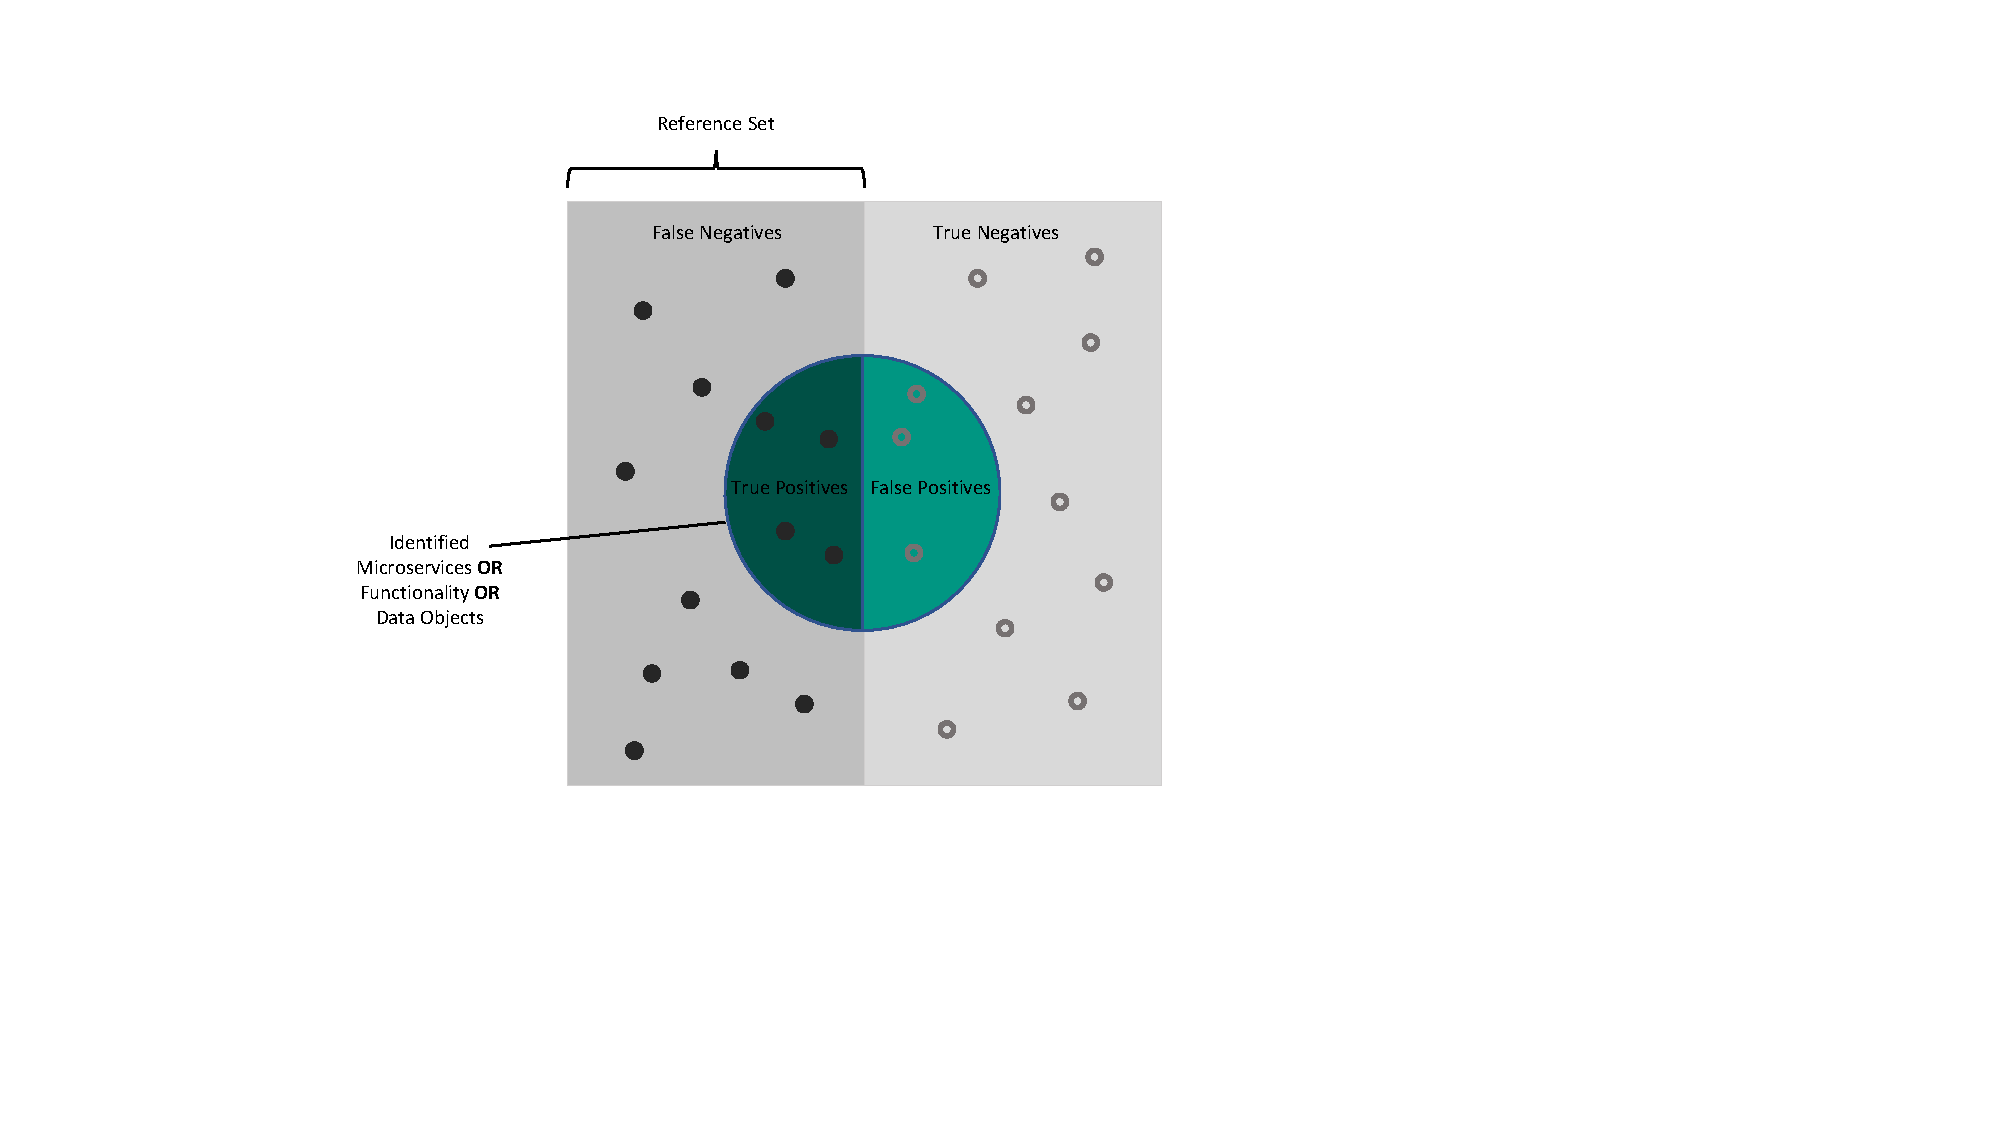
\includegraphics[ trim={7cm 5.5cm 8cm 0.5cm}, scale =1]{img/PrecisionRecall.pdf}
	\caption{Precision and Recall for Microservices}
	\label{fig:PrecisionRecall}
\end{figure}







\section{Reference Sets}
\label{sec:Evaluation:ReferenceSets}
To evaluate the approach, the identified set of microservices (cf. Sec.\ref{sec:Evalutation:Results}) is compared to two alternative decompositions of CoCoME: First, a decomposition proposed in the paper \textit{Identifying Microservices Using Functional Decomposition} \cite{FunctionalDecompositionHeinrich} and second, a set of microservices which we manually identified. \\



\subsection{Reference Set 1: Functional Decomposition Approach}
\textit{Identifying Microservices Using Functional Decomposition} \cite{FunctionalDecompositionHeinrich} is a systematic approach to find a appropriate partition of a system into microservices. This paper emerged as a result of the collaboration of the Academic College Tel-Aviv Yafo, the Karlsruhe Institute of Technology and the Southwest University China and uses CoCoME as demonstrator as well.\\
As depicted in Sec.\ref{sec:stateOfTheArt:approaches}, Tyszberowicz et al. utilize the use case specifications of CoCoME \cite{CoCoMEOld} as input for their decomposition approach. Several external tools are used to extract verbs an nouns from the use cases that serve as \textit{system operations} and \textit{state variables}. Irrelevant noun, verbs and synonyms are eliminated via brainstorming. The relationships between the aforementioned concepts are stored in a relation table. A relation exists, if a \textit{system operation} reads or updates a \textit{state variable}. Thereupon, the relation table is visualized as a weighted graph, which enables to identify clusters of dense relationships. Each cluster serves as a microservice candidate.\\
As mentioned in Sec.\ref{sec:stateOfTheArt:comparison}, the compulsory and non-trivial revision of nouns and verbs to eliminate synonyms etc. is a substantial disadvantage. 


Regarding the evaluation, Tyszberowicz et al. claim that their approach identifies good microservices for a microservice-based system decomposition of CoCoME. The aforementioned evaluation includes a comparison to three independent software projects that implemented CoCoME. Two groups identified, apart from the naming, a similar set of microservices. The third group identified a more detailed decomposition of CoCoME, but a revision reveals that the additional microservices are only a refinement of the proposed microservices. \\
However, the evaluation lacks profundity: Microservices are only compared on a more abstract level, as is not checked whether functionality and data objects are assigned to the correct microservice. The following microservices are identified: 



\begin{multicols}{2}
	\textbf{Sale}
	\begin{flushleft}
		\begin{itemize}[noitemsep]
			\item Handle Sale
			\item Handle Payment
			\item Identify stock Item
			\item \textbf{Data objects}: -  
		\end{itemize}
	\end{flushleft}
	
	
	\vfill
	\columnbreak
	\textbf{ProductList}
	\begin{flushleft}
		\begin{itemize}[noitemsep]
			\item Create orders
			\item Change price
			\item \textbf{Data Objects}: product
			
			
		\end{itemize}
	\end{flushleft}
	
\end{multicols}




\begin{multicols}{2}
	\textbf{StockOrder}
	\begin{flushleft}
		\begin{itemize}[noitemsep]
			\item Create stock report
			\item Handle inventory
			\item \textbf{Data objects}: stockItem, order
		\end{itemize}
	\end{flushleft}
	
	
	\vfill
	\columnbreak
	\textbf{Reporting}
	\begin{flushleft}
		\begin{itemize}[noitemsep]
			\item Create delivery report
			\item Handle deliveries
			\item \textbf{Data Objects}: - 
			
		\end{itemize}
	\end{flushleft}
\end{multicols}



\subsection{Reference Set 2: Manual Decomposition}
In the course of this thesis, we implemented a microservice-based version of CoCoME. The microservice identification process itself was terminated before the literature review for the thesis started. Moreover, we were not aware of the microservice decomposition proposed by Tyszberowicz et al. \cite{FunctionalDecompositionHeinrich} by the time we identified possible microservice candidates. So, the process was non-biased. \\
The identification process itself was conducted manually and supported by the previous knowledge of the CoCoME domain. Once more, the time consuming and difficult identification process clarified the necessity of a structured and formal approach to identify microservices. Beside the use case specification, we used a monolithic implementation of CoCoME (the Hybrid Cloud-based Variant \cite{CoCoMETechnical}) as additional information resource to discover requirements, functionality and dependencies. Subsequently, the system was decomposed into loosely coupled and high cohesive microservices. \\
The following four microservices were identified:




\begin{multicols}{2}
	\textbf{Stores- and Sale}
	\begin{flushleft}
		\begin{itemize}[noitemsep]
			\item Handle sale
			\item Handle payment
			\item Manage express checkout
			\item Exchange products
			\item Identify stock items
			\item Handle inventory
			\item Change price
			\item Handle stores
			\item Handle enterprises
			\item Handle deliveries
			\item \textbf{Data objects}: stockItem, store, enterprise
		\end{itemize}
	\end{flushleft}
	
	
	\vfill
	\columnbreak
	\textbf{Product}
	\begin{flushleft}
		\begin{itemize}[noitemsep]
			\item Show products
			\item Create products
			\item Show suppliers
			\item Create suppliers
			\item \textbf{Data Objects}: product, supplier
		
		
		\end{itemize}
	\end{flushleft}

\end{multicols}




\begin{multicols}{2}
	\textbf{Order}
	\begin{flushleft}
		\begin{itemize}[noitemsep]
			\item Show orders
			\item Create orders
			\item \textbf{Data objects}: order
		\end{itemize}
	\end{flushleft}
	
	
    	\vfill
	\columnbreak
	\textbf{Reports}
	\begin{flushleft}
		\begin{itemize}[noitemsep]
			\item Create delivery report
			\item Create stock report
			\item \textbf{Data Objects}: report  
	
		\end{itemize}
	\end{flushleft}
\end{multicols}






\subsection{Differences between both sets}
The reference sets contain the same amount of microservices. Apart from the naming, those services are similar: One is responsible for the sale process, another one handles products, the third one is responsible for the orders and the last one is in charge of the reporting. \\
Nevertheless, the two differ from each other in regard to the functionality and data objects. Obviously, \textit{Reference Set 1} features nine functionalities and three data objects whereas \textit{Reference Set 2} contains 18 functionalities and seven data objects. It is important to note that all functionalities and data objects of the first reference set are part of the second one. Since the second reference set corresponds to a real implementation, it can be assumed that the first set is not complete. \\
Furthermore, both sets differ in the distribution of functionality and data objects among services. For instance, in \textit{Reference Set 1} the data object \textit{stockItem} is divided into the order microservice, whereas in \textit{Reference Set 2} it is divided into the sale's microservice. To provide another example, the functionalities \textit{Create Stock Report} and \textit{Create Delivery Report} are distributed differently: In the first reference set, \textit{Create Stock Report} is part of the report microservice and \textit{Create Delivery Report} is part of the order microservice whereas in the second reference set, both functionalities belong to the report service. \\




\section{Precision and Recall Measurement}
\label{sec:Evalutation:PrecisionAndRecallMeasurement}
In this section, the precision and recall metric (cf. Sec.\ref{sec:Evaluation:Metrics:sPrecRecall}) for the results of the approach (cf. Sec.\ref{sec:SolutionApplication:ExtractMicroserviceCandidates}) is calculated using the reference sets described in Sec.\ref{sec:Evaluation:ReferenceSets}. 
For each reference set, the precision and recall instances are i) identified microservices, ii) identified functionality offered by a microservice and iii) identified data objects administered by a microservice. 

\subsection{Reference Set 1}

\textbf{Microservices} The approach identified three services, where \textit{Microservice 1} is similar to \textit{Sale} and \textit{Microservice 2} is comparable to \textit{Reporting}. \textit{Microservice 3}, on the other hand, can neither be clearly assigned to \textit{StockOrder} nor to \textit{ProductList}, since it unites the functionalities of both. More specifically, \textit{Microservice 3} is a more coarse-grained microservice that consists of \textit{StockOrder} and \textit{ProductList}. Therefore it can be concluded that three out of four microservices were successfully identified, and none of the identified microservices are incorrect. 

\hspace{1cm}
\noindent
\begin{minipage}{.4\linewidth}
		\vspace{0.5cm}
	\flushleft

		
	$Recall_{microservice}=\dfrac{3}{4} = 0.75  $
		\vspace{0.5cm}
	
\end{minipage}%
\begin{minipage}{.5\linewidth}
	\vspace{0.5cm}
	\flushleft

		
	$Precision_{microservice}=\dfrac{3}{3} = 1  $
		\vspace{0.5cm}
	
\end{minipage}

\noindent
\textbf{Functionality} Since \textit{Microservice 3} consists of the microservices \textit{StockOrder} and \textit{ProductList}, functions that appear in this microservice and in either of the other two are regarded to be successfully identified. With this in mind, the results are as follows: The reference set counts nine functionalities. The approach identified 13 functionalities, from which five are assigned to the right service. Hence, the precision and recall values are:

\hspace{1cm}
\noindent
\begin{minipage}{.4\linewidth}
	\vspace{0.5cm}
	\flushleft
	
	
	$Recall_{functionality}=\dfrac{5}{9} \approx 0.56  $
	\vspace{0.5cm}
	
\end{minipage}%
\begin{minipage}{.5\linewidth}
	\vspace{0.5cm}
	\flushleft
	
	
	$Precision_{functionality}=\dfrac{5}{13} \approx 0.38  $
	\vspace{0.5cm}
	
\end{minipage}


\noindent
\textbf{Data Objects} Regarding \textit{Microservice 3}, the same line of reasoning is applied to the identified data objects: The reference set counts three data objects. The approach identified seven, from which 2 are assigned to the right service. In this case, the precision and recall values are:


\hspace{1cm}
\noindent
\begin{minipage}{.4\linewidth}
	\vspace{0.5cm}
	\flushleft
	
	
	$Recall_{dataObject}=\dfrac{2}{3} \approx 0.67  $
	\vspace{0.5cm}
	
\end{minipage}%
\begin{minipage}{.5\linewidth}
	\vspace{0.5cm}
	\flushleft
	
	
	$Precision_{dataObject}=\dfrac{2}{7} \approx 0.29  $
	\vspace{0.5cm}
	
\end{minipage}





\subsection{Reference Set 2}



\textbf{Microservices} As described in Sec.\ref{sec:Evaluation:ReferenceSets}, both reference sets contain similar microservices, which differ only by the names at microservice level. The functionalities and data objects, however, are different. Hence, the precision and recall value are identical in regard to identified microservices:

\hspace{1cm}
\noindent
\begin{minipage}{.4\linewidth}
	\vspace{0.5cm}
	\flushleft
	
	
	$Recall_{microservice}=\dfrac{3}{4} = 0.75  $
	\vspace{0.5cm}
	
\end{minipage}%
\begin{minipage}{.5\linewidth}
	\vspace{0.5cm}
	\flushleft
	
	
	$Precision_{microservice}=\dfrac{3}{3} = 1  $
	\vspace{0.5cm}
	
\end{minipage}

\noindent
\textbf{Functionality} Again \textit{Microservice 3} is considered to be a coarse grained union of the microservice \textit{Product} and \textit{Order}. In this case, the reference set counts 18 functionalities. The approach identified 13 functionalities, from which 12 are assigned to the right service. Hence, the precision and recall values are:

\hspace{1cm}
\noindent
\begin{minipage}{.4\linewidth}
	\vspace{0.5cm}
	\flushleft
	
	
	$Recall_{functionality}=\dfrac{12}{18} \approx 0.67  $
	\vspace{0.5cm}
	
\end{minipage}%
\begin{minipage}{.5\linewidth}
	\vspace{0.5cm}
	\flushleft
	
	
	$Precision_{functionality}=\dfrac{12}{13} \approx 0.92  $
	\vspace{0.5cm}
	
\end{minipage}


\noindent
\textbf{Data Objects} The reference set counts seven data objects. The approach identified seven, from which 5 are assigned to the right service. In this case, the precision and recall values are:


\hspace{1cm}
\noindent
\begin{minipage}{.4\linewidth}
	\vspace{0.5cm}
	\flushleft
	
	
	$Recall_{dataObject}=\dfrac{5}{7} \approx 0.71  $
	\vspace{0.5cm}
	
\end{minipage}%
\begin{minipage}{.5\linewidth}
	\vspace{0.5cm}
	\flushleft
	
	
	$Precision_{dataObject}=\dfrac{5}{7} \approx 0.71  $
	\vspace{0.5cm}
	
\end{minipage}

\section{Results}
\label{sec:Evalutation:Results}
The measurement of the precision and recall metric in the previous section gives information about the accuracy of the approach. Each of the identified microservices is also represented in the reference sets, which leads to a maximum precision of \textit{1}. Due to the coarse-grained \textit{Microservice 3} the recall is at 0.75. However, it has to be noticed that the approach did not produce any incorrect  microservices. \\
Functionality... Unteschiede in den Sets...



Nichts falsch idnentifiziert 



\section{Threats to Validity}
\label{sec:Evalutation:ThreatsToValidity}
* Das abstrahieren der FUnktionalität biased by the outcome
* Zusätzliche infos aus monolith
* Zusammenlegen oder Product Strictly speaking, only two of the four services were identified.  --> Hätten wir das nciht gemaht wäre Ergebnis verzerrt, da es ja trotzdem richtig zugeordnet wurde --> Ohne diese Annahme...

*Intern: wie ist die studie designed; können die Ergebnisse auch anders interpretiert weden --> Sy<stematische fehler, bias...
*Extern: Wurde der Ansatz so entwickelt dass er auf CoCoME passst...


